\chapter{Preliminary}

\subsubsection{Problem Formulation}
\label{sec:problem_formulation}

The input to the pipeline will be a standard image, which will first be converted to black and white, cropped into a square, and then its pixel values will be scaled to the [0,1] range. In addition, we will invert the black and white values. This is because, in traditional computer graphics, white is represented as 1 and black as 0, but our problem involves drawing thin black edges. Swapping these values promotes sparsity, which helps reduce computation time. It also aligns better with our approach, since we can \textit{add} lines together to build up the image. Lastly, we will flatten the image row-wise, and the result will be denoted as a column vector \(b \in \mathbb{R}^{m^2}\), where \(m\) is the width or height of the image.

Let \(N\) denote the number of pegs used in our computation, and let \(n = \binom{N}{2}\) the total number of possible lines that can be drawn. With this in mind, we define each matrix \(A_i\) as the matrix representing the \(i\text{-th}\) line drawn on the canvas. The final matrix \(A \in \mathbb{R}^{m^2, \space n}\) is constructed such that each column corresponds to the flattened, row-wise version of a matrix \(A_i\). This matrix \(A\) will be used in the computations that follow.

Finally, let \(x \in \mathbb{R}^n\) or \(x \in \{0, 1\}^n\) if the output vector of our solution is binary. Here, \(x_i\) indicates how much we choose to draw the \(i\text{-th}\) line, or whether we choose to draw it at all, in the binary case.

With all of the above defined, we can state our objective as minimizing the error between the string art configuration and the input image using a standard least squares formulation with the 2-norm:

\begin{equation}
\min{\| A \cdot x - b \|^2}
\label{eq:least_squares}
\end{equation}

Given the fact that the intersection of lines can create pixel values \(\geq1\) we will use a clamping function when computing the image:

\begin{equation}
y = C(Ax), \quad
C : \mathbb{R}_+^{m, \ m} \rightarrow [0, 1]^{m, \ m}, \quad
C(x) = \min(x, 1)
\label{clamping_operator}
\end{equation}

It is important to note that there exists a discrepancy in a computers perception of a \enquote{qualitative} image and the human eye. In the formula above, the computer will consider that the image with the lowest residual is the highest quality one.

\begin{figure}[H]
    \centering
    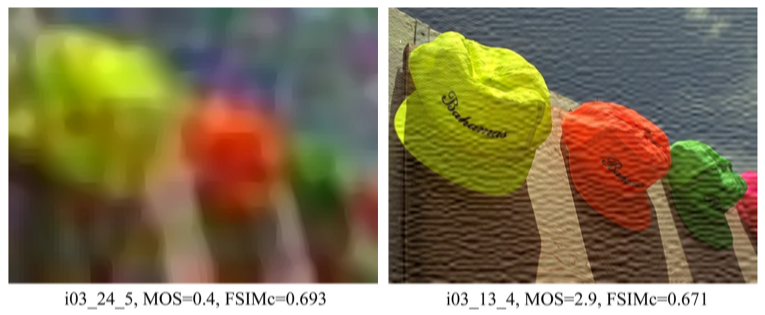
\includegraphics[width=0.66\linewidth]{perceptual_image_quality.png}
    \caption{Image taken from the paper \cite{perceptual_image_quality} which showcases the discrepancy between the errors given by computers and humans.}
    \label{fig:perceptual_image_quality}
\end{figure}

This phenomenon can be observed in the figure above, where the image on the left, despite having a higher FSIMc score \cite{fsimc} (the higher the better), has a lower MOS\footnote{For more details about the Mean Opinion Score (MOS), see the article on \href{https://en.wikipedia.org/wiki/Mean_opinion_score}{Mean Opinion Score (MOS)}}. This indicates that the majority of people perceived the image on the right as being of higher quality, which contradicts the result given by the computer.

\subsubsection{Peg Placement}

To place the pegs equidistantly on a circle, we used the following parametric equation of a circle.

For a circle centered at \((x_c, y_c)\) with radius \(r\) and \(N\) pegs:

\[
\begin{aligned}
x_k &= x_c + r \cdot \cos\left( \frac{2\pi k}{N} \right), \\
y_k &= y_c + r \cdot \sin\left( \frac{2\pi k}{N} \right),
\end{aligned}
\quad \text{for } k = 0, 1, 2, \dots, N - 1
\]

This placement ensures that the directions of lines connecting peg pairs are distributed uniformly over the angular domain. This is particularly important due to the Fourier Slice Theorem\footnote{For the connection between Radon and Fourier transforms, see the article on \href{https://en.wikipedia.org/wiki/Projection-slice_theorem}{Fourier Slice Theorem}}, which connects the Radon transform with the 2D Fourier transform: equidistant angular sampling allows for more accurate coverage of the frequency domain and, in turn, better image approximation through string lines.

\subsubsection{Line Rendering}

For rendering lines in the matrix representation, we initially used the Bresenham algorithm\footnote{For a detailed implementation of the algorithm, see the article on \href{https://en.wikipedia.org/wiki/Bresenham\%27s\_line\_algorithm\#Algorithm}{Bresenham's Line Algorithm}}, and later switched to the anti-aliased Xiaolin-Wu algorithm\footnote{For a detailed implementation of the algorithm, see the article on \href{https://en.wikipedia.org/wiki/Xiaolin_Wu\%27s_line_algorithm}{Xiaolin Wu's line algorithm}}.
